%Copyright 2014 Jean-Philippe Eisenbarth
%This program is free software: you can
%redistribute it and/or modify it under the terms of the GNU General Public
%License as published by the Free Software Foundation, either version 3 of the
%License, or {at your option} any later version.
%This program is distributed in the hope that it will be useful,but WITHOUT ANY
%WARRANTY; without even the implied warranty of MERCHANTABILITY or FITNESS FOR A
%PARTICULAR PURPOSE. See the GNU General Public License for more details.
%You should have received a copy of the GNU General Public License along with
%this program.  If not, see <http://www.gnu.org/licenses/>.

%Based on the code of Yiannis Lazarides
%http://tex.stackexchange.com/questions/42602/software-requirements-specification-with-latex
%http://tex.stackexchange.com/users/963/yiannis-lazarides
%Also based on the template of Karl E. Wiegers
%http://www.se.rit.edu/~emad/teaching/slides/srs_template_sep14.pdf
%http://karlwiegers.com
%\documentclass[letterpaper,10pt]{article}
\documentclass{scrreprt}
\usepackage{listings}
\usepackage{underscore}
\usepackage[bookmarks=true]{hyperref}
\usepackage[utf8]{inputenc}
\usepackage[english]{babel}
\usepackage{graphicx}
\usepackage{amssymb}
\usepackage{amsmath}
\usepackage{amsthm}
\usepackage{afterpage}

\usepackage{alltt}
\usepackage{float}
\usepackage{color}
\usepackage{url}

\usepackage{enumitem}

\usepackage{geometry}

\usepackage{titling}
\usepackage{rotating}
\usepackage{pgfgantt}
\usepackage{graphicx}
\usepackage{xcolor}
\usepackage{anyfontsize}

\ganttset{group/.append style={orange},
milestone/.append style={red},
progress label node anchor/.append style={text=red}}

\newcommand\blankpage{
    \null
    \thispagestyle{empty}
    \addtocounter{page}{0}
    \newpage}

\geometry{textheight=8.5in, textwidth=6in}
\hypersetup{
    bookmarks=false,    % show bookmarks bar?
    pdftitle={Software Requirement Specification},    % title
    pdfauthor={Jean-Philippe Eisenbarth},                     % author
    pdfsubject={TeX and LaTeX},                        % subject of the document
    pdfkeywords={TeX, LaTeX, graphics, images}, % list of keywords
    colorlinks=true,       % false: boxed links; true: colored links
    linkcolor=blue,       % color of internal links
    citecolor=black,       % color of links to bibliography
    filecolor=black,        % color of file links
    urlcolor=purple,        % color of external links
    linktoc=page            % only page is linked
}%
\def\myversion{1.0 }
\date{}
%\title
\usepackage{hyperref}
\begin{document}

\begin{titlingpage}
	\begin{flushright}
		\rule{16cm}{5pt}\vskip1cm
		\begin{bfseries}
			\Huge{Design Document}\\
			\vspace{1.0cm}
			Deep Learning on Embedded Platform\\
			\vspace{1.0cm}
			\LARGE{Version \myversion}\\
			\vspace{1.0cm}
			Prepared by Christopher Johnson, Luay Alshawi, Gabe Morey\\
			\vspace{1.0cm}
			CS 461 Fall 2016\\
			\vspace{1.0cm}
			\today\\
		\end{bfseries}
	\end{flushright}
	\begin{abstract}
	This document goes over the design decision made for our Deep Learning on Embedded Platform project.
	In it we will explain our approach, provide detailed information about why we designed it a certain way, and explain our expected outcome.
	\end{abstract}
\end{titlingpage}
\afterpage{\blankpage}

\tableofcontents

\chapter{Overview}
\section{Scope}

This document outlines the design of a system for teaching a deep learning neural network how to play the game Galaga.
The sections of this document will outline the system details, setup, and all things necessary to understand how and why the project is designed.
Hardware required, API's used, and setup will be detailed as part of the project design.

This project is to be used to produce a training course for NVIDIA's Deep Learning Institute.
After the project is complete it will be handed off to NVIDIA for the purposes of accomplishing this goal.

\section{Purpose}

The main aim of this document is to give others a thorough enough understanding of the project and its design.
The reader of this document should walk away able to understand how the system works and why it was designed this way.
The document must be thorough enough for NVIDIA to recreate the project and package the design into a training course on deep learning.


\chapter{Definitions}

3.1 Neural Network: A multilayered graph structure containing nodes, referred to as neurons, and weights that affect how likely the node is to be chosen when confronted with a decision. The weights of nodes are decided through training the network, and a traversal of the graph acts as a large chain of decisions as the neural network is confronted with situations.

3.2 Deep Learning: Using a layered neural network constructed by GPU processing to teach a computer how to accomplish a specific task.

3.3 Convolutional Neural Network: A neural network specifically designed to take images as input. It uses convolutional layers to process the image into a more manageable chunk of data and extracts the information relevant to the network.

3.4 Caffe: A code framework that allows for complex mathematical operations that are required for training a neural network.

3. API: Application Programming Interface

3. Jetson TX1: Quad core embedded system designed for power efficiency and deep learning projects

3. OS: Operating system

\chapter{Design}

\section{Introduction}

\section{Development viewpoint}%Gabe

\subsection{Set up image dataset}%Luay

\section{Neural network setup}%Gabe

\section{Data viewpoint}%Luay

\subsection{Image processing}%Luay

\subsection{Neural training methods}%Gabe

\subsection{Data visualization}%Chris

We also needed to figure out how we were going to display the results of each round.
We decided it would be best to have a summary graphical display of the data at the end of the playthrough.
Once the program runs out of lives a screen will appear graphing statistics about the machines performance.
These statistics will include things such as how long the machine lasted, how many levels it completed, which enemies or objects took away the most lives, and so on.
Having detailed and easily readable data is key to knowing how to train the machine as we progress through the project.

\section{Hardware viewpoint}%Chris

While working with the Jetson TX1 there are several things that we needed to decide.
These included our methods to communicate with our client, and the hardware used with the Jetson.
Choosing out hardware was key to determining how each piece would fit into the design.

For communication purposes, our team decided to stick with using skype.
We will conduct regular meetings with our client and continue using skype, which everyone is familiar with.
Skype will allow us to video call as well, in case any visuals need to be explained.

Our project will actually need to be able to control the game.
Inputs from the neural net need to be received by the game so that it can be played.
To do this we decided not to use the standard keyboard.
Using a keyboard requires a lot of additional coding to map the Jetson to the controls.
Instead we decided to find a game controller that we will hardwire to the Jetson TX1.

\subsection{Hardware setup}%Chris

A game controller will significantly reduce the work load because it will already contain a lot of built in functionality that we need to connect it to the Jetson.
The Jetson will be able to control the game using the controller's built in functionality.

\begin{figure}
  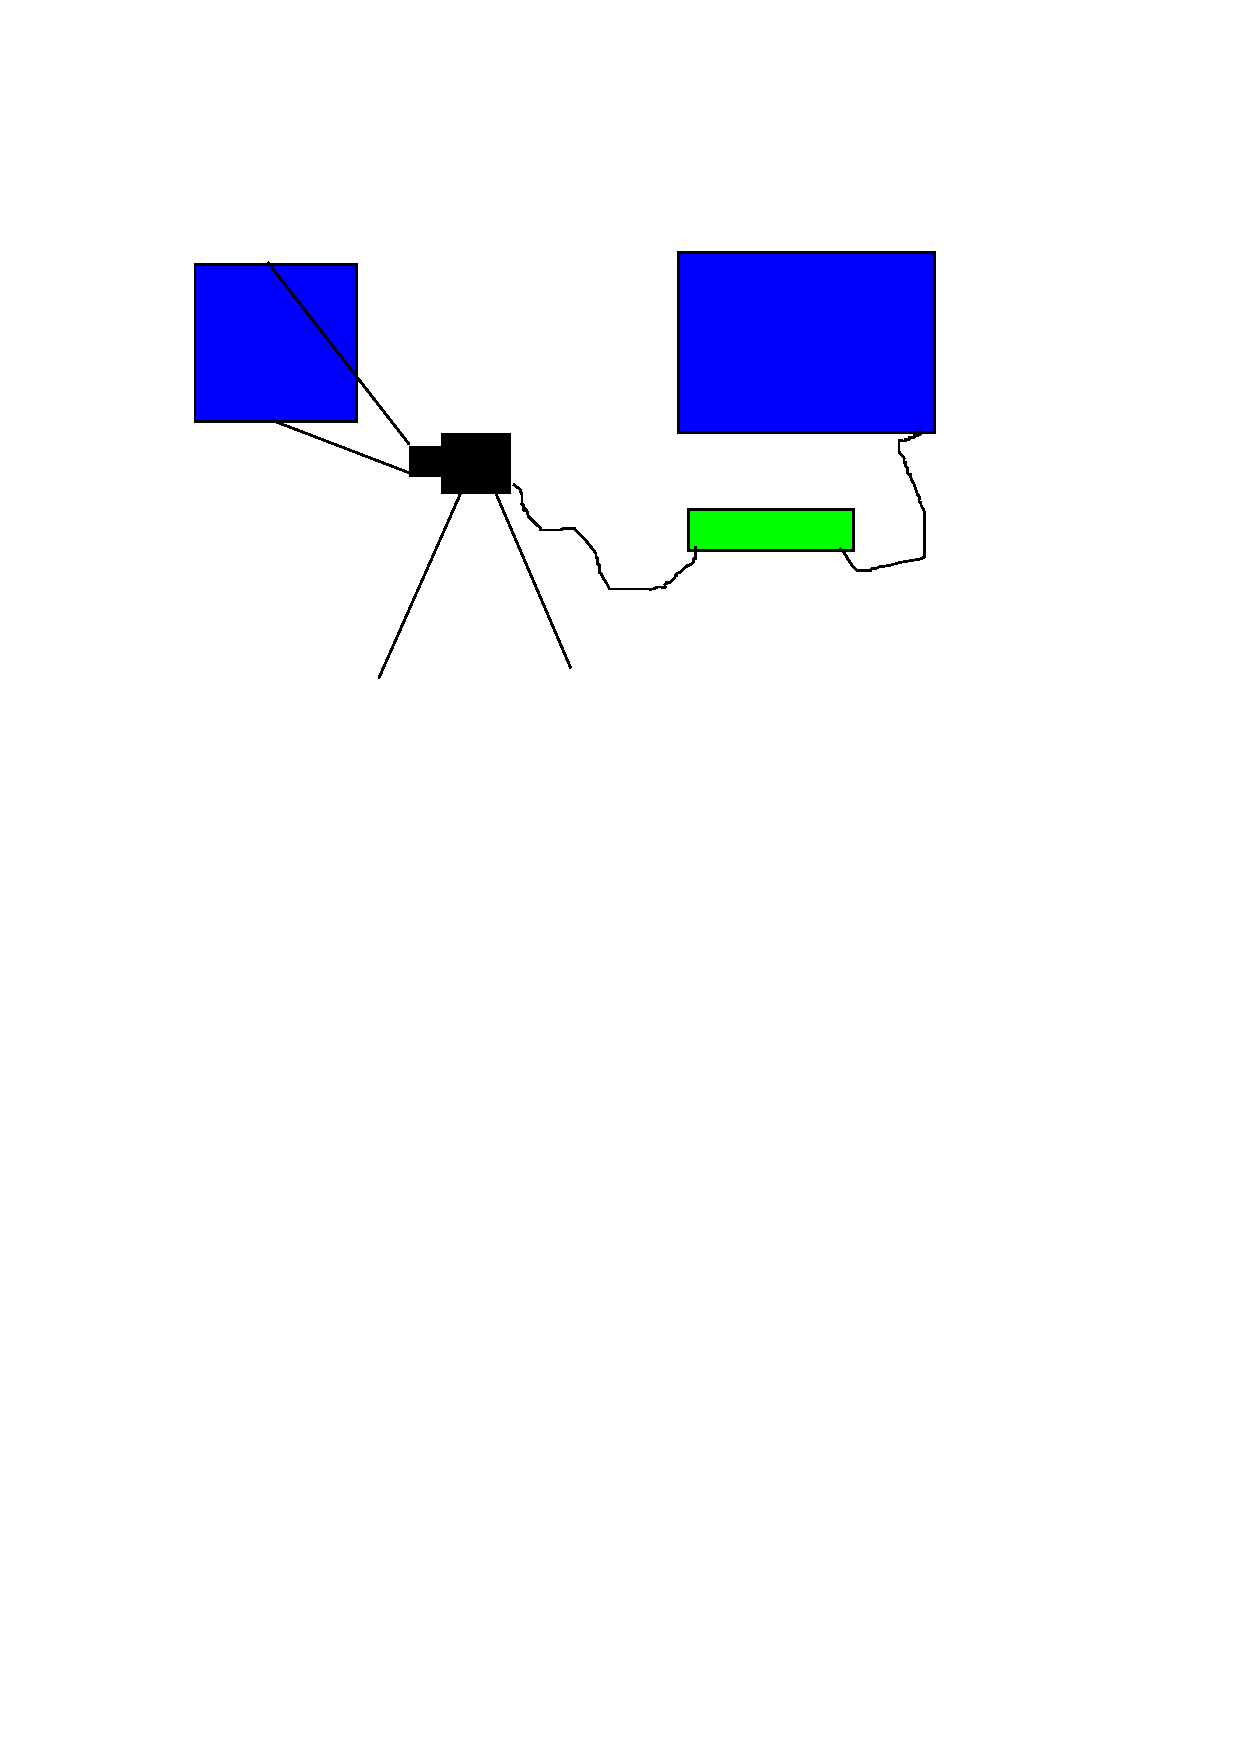
\includegraphics[width=\linewidth,natwidth=50,natheight=100]{design.PNG}
  \caption{Hardware Layout}
  \label{fig:design1}
\end{figure}
Figure \ref{fig:design1} shows the basic layout.

Since the Jetson has to learn how to play the game it needs to be able to see the game.
For this we decided to use the camera sent to us by our client.
This was the simplest option seeing as we can connect the camera directly to the Jetson.
The camera will be connected to the Jetson and aimed at another screen displaying the game.
The Jetson will first be trained by being given the video input to recognize and characterize objects within the game.
We will set up tables so that the neural net will be able to store information such as the locations of objects.
Once those things are set up it will be able to train itself by playing the game using the controller.
It will base its decisions on the table of information that it stores and will increasingly be able to survive the game longer.
Eventually it will learn to respond to certain patterns in the table in order to become better at the game.

\chapter{Conclusion}

\end{document}